\section{Taking derivatives by the method of Backwards Differentiation}
A computer algorithm is embodied in a list of assignment statements. It can be thought of as an ordered list of recursions where each subsequent line in the list is a function of the preceding lines whose values have been stored and are retrievable when needed later. Taking derivatives of the subsequent quantities can be done line at a time. There are two methods that one can consider -- forwards differentiation where one starts at the beginning of the list and works down towards the end or starts are the bottom (assuming all the intermediate quantities are retrievable from storage) and works back towards the beginning of the list. Let us set up the framework in which to define both methods of differentiation and how they compare. \\

Consider an ordered list of $r$ recursions
\begin{align*}
1.~~h_1 &= h_1(\Omega_1)\\
2.~~h_2 &= h_2(\Omega_2)\\ 
             &\vdots\\
r.~~h_r &= h_r(\Omega_r)\\
\end{align*}where $\Omega_k$ represents the set of all previously computed quantities and the parameters, $\bf x$ which the algorithm takes as input. Now for the $k$th line we can express this set
of parameters as a union of all the previously computed items: $\Omega_k \subseteq {\bf x} \cup \{ h_i: ~i<k\}$ together with the list of parameters $\bf x$. If there are $n$ such parameters we can implicitly include them in the list of recursions symbolically as $h_1 = x_1, h_2 = x_2, \hdots, h_n = x_n$, so we may assume $\Omega_k \subseteq \{h_i: i < k\}$. The objective is to compute the derivatives of the final assignment statement (or any of its predecessors) in terms of the parameters list, i.e., we wish to have a general method to compute $\partial h_j/\partial {\bf x}$ for any $j \le r$.\\

The method of Forwards Differentiation proceeds by a straightforward application of the chain rule as follows: 
\begin{align*}
1.~~ h_1 &= h_1(\Omega_1), ~~ {\partial h_1\over \partial {\bf x}} = \sum_{h_i\in \Omega_1}\, {\partial h_1\over\partial h_i} {\partial h_i\over\partial {\bf x}}\\
2.~~ h_2 &= h_2(\Omega_2), ~~ {\partial h_2\over \partial {\bf x}} = \sum_{h_i\in \Omega_2}\, {\partial h_2\over\partial h_i} {\partial h_i\over\partial {\bf x}}\\
3.~~ h_3 &= h_3(\Omega_3), ~~ {\partial h_3\over \partial {\bf x}} = \sum_{h_i\in \Omega_3}\, {\partial h_3\over\partial h_i} {\partial h_i\over\partial {\bf x}}\\
               &\vdots~~~~~~~~~~~~~~~~~~~~~~~~~~~~~~~~~~~\vdots\\
r.~~ h_r  &= h_r(\Omega_r),   ~~ {\partial h_r\over \partial {\bf x}} = \sum_{h_i\in \Omega_r}\, {\partial h_r\over\partial h_i} {\partial h_i\over\partial {\bf x}}\\
\end{align*}By extension second derivatives are found similarly. It should be pointed out here that the process of gathering up the full set of derivatives with respect to all the parameters in the list
$\bf x$ requires $n$ forward passes through the above differentation algorithm. The is the nature of Forwards Differentiation.\\


The method of Backwards Differentiation or Adjoint Differentiation proceeds by implementing a work array whose length is the same as the list of recursions including the parameters and starting at the botton of the list and working upwards towards the top. The rules for Backwards Differentiation are captured in the following:

\begin{align*}
1. ~~ & \hbox{Initialize}\ F_j = 0, \hbox{for}\ i<r \hbox{ and set } F(r) = 1\\
2. ~~& F_i = F_i + F_j (\partial h_k/\partial h_j) \hbox{ for all } i \hbox{ such that } h_j \in \Omega_k, ~~ k = r, r-1, \hdots, n+1\\
3. ~~&\hbox{Then } \partial h_r/\partial h_i = F_i, ~i = 1,2\hdots r.\\
\end{align*}

We need to determine $i$ and $k$ going backward and compute $\partial h_k/\partial h_i$ dynamically from $h_1, h_2, \hdots, h_r$. There are also various tools available to 
implement such an algorithm automatically such as ADIFOR for FORTRAN and AutoDiff for MATLAB, but for the projects that I have applied this method to, the number of lines of code
is not prohibitive to code the above algorithm ``by hand.'' The main point of Backwards Differentiation is that the work vector $F$ stores the intermediate results in an efficient 
manner and would otherwise require a large amount of computation to expand the whole differentiation procedure using formulas for each derivative. Also, one backwards pass through the algorithm produces the entire gradient of $h_r$ (or any other intermediate computation). \\
\begin{figure}[hptp]
\begin{center}
   \resizebox{0.6\linewidth}{0.5\linewidth}{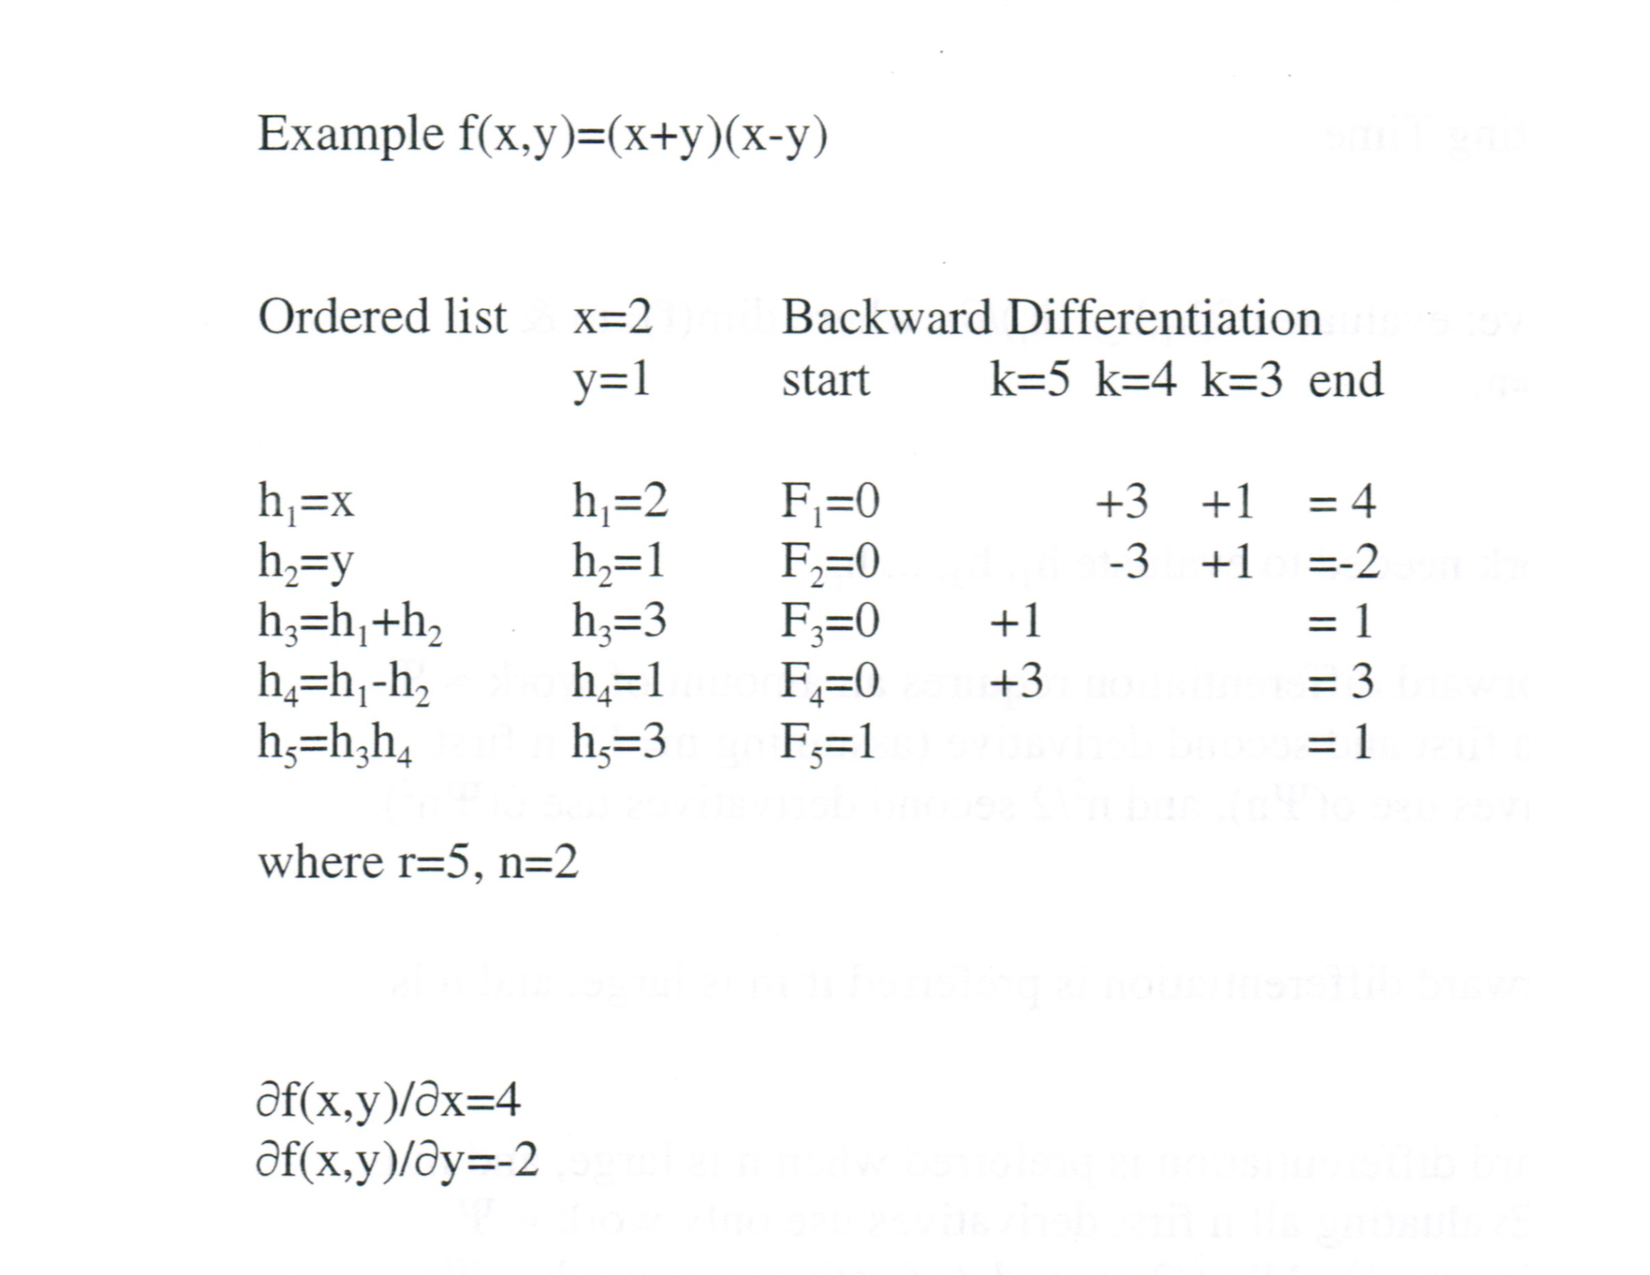
\includegraphics{BackwardsDifferentiationExample.pdf}}
   \caption{Example of Backwards Differentiation}
   \label{fig:BackwardsDifferentiation} 
\end{center}
\end{figure}

Second derivatives can be obtained by applying backwards differentiation twice, or by applying backwards differentiation and forwards differentiation in either order. Three work vectors each of length 
$r$ (the length of the list of recursions in the algorithm) are required. Let $\bf F$ be provided by the backwards differentiation algorithm above to compute all the derivatives of $h_r$. Let $\bf Q$ and $\bf S$ each be arrays also of length $r$. Then second derivatives can be computed using the following algorithm: 

\begin{align*}
1.~~ & \hbox{Initialize } Q_v = 1, Q_j = 0 \hbox{ and } v\in \{1,2,\hdots, n\} \hbox{ and } S_j = 0, \forall j = 1,2, \hdots, r\\
2.~~ & Q_k = Q_K + Q_i (\partial h_k/ \partial h_i), h \in \Omega_k; \\
        & S_j = S_j + Q_i F_k (\partial^2 h_k/\partial h_i \partial h_j), ~ h_i, h_k \in \Omega_k, ~ k = n+1, n+2, \hdots, r\\ 
3.~~ & S_j = S_j + S_k (\partial h_k/\partial h_i), ~h_j \in \Omega_k,~ k = r, r-1, \hdots, n+1\\
4.~~ & \hbox{Then } \partial^2 h_r/\partial x_v \partial x_j = S_i, ~ i = 1,2,\hdots,n\\
\end{align*}Note that $\bf Q$ is calculated by the forward differentiation equations and Step 3 is the first derivatives by backwards differentiation algorithm. This is an example of applying forwards differentation to the backwards differentiation algorithm in order to calculate the 2nd derivatives of $h_r$ with respect to the parameter set $\bf x$. As mentioned, one can also apply backwards differentation twice or forwards differentiation followed by backwards differentiation. The above keeps the bookkeeping aligned in the sense that all three work vectors $\bf F$, $\bf Q$ and $\bf S$ have the same length.

